\documentclass[11pt,aspectratio=169]{beamer}

% -------------------- THEME & LAYOUT --------------------
\usetheme{Madrid}
\usecolortheme{dolphin} % base color scheme
\usefonttheme{professionalfonts}
\setbeamercovered{transparent}
\setbeamertemplate{navigation symbols}{}   % remove navigation buttons
\setbeamertemplate{caption}[numbered]      % numbered captions
\setbeamertemplate{itemize items}[triangle]
\setbeamersize{text margin left=1.2cm,text margin right=1.2cm} % adjust to taste
% -------------------- GLOBAL FONT SETTINGS --------------------

% 1. Force the base beamer font to small
\setbeamerfont{normal text}{size=\small}

% 2. Force math environments to follow the "small" font size
\setbeamerfont{math text}{size=\small}
\setbeamerfont{equation}{size=\small}

% 3. Redefine \normalsize itself 
% This ensures equations and lists (which look for \normalsize) use  instead.
\let\oldnormalsize\normalsize
\renewcommand{\normalsize}{\oldnormalsize\small}

% 4. Ensure lists also stay small
\setbeamerfont{itemize/enumerate body}{size=\small}
\setbeamerfont{itemize/enumerate subbody}{size=\small}

% -------------------- FONTS & TYPOGRAPHY --------------------
\usepackage[T1]{fontenc}
\usepackage[utf8]{inputenc}
\usepackage{newpxtext,newpxmath} % Palatino-like font & math
\usepackage{microtype}

% -------------------- MATH, TABLES & GRAPHICS --------------------
\usepackage{amsmath,amssymb,amsfonts,mathtools}
\usepackage{bm,booktabs,siunitx,graphicx}
\graphicspath{{./}{./figures/}}
\renewcommand{\theequation}{1.\arabic{equation}}

% -------------------- UTILITIES --------------------
\usepackage{appendixnumberbeamer}
\usepackage{ragged2e}
\usepackage{xspace}
\usepackage{csquotes}
\usepackage{xcolor}

% -------------------- HYPERREF --------------------
\hypersetup{
  colorlinks=false,
  pdfauthor={Francesca},
  pdftitle={Chapter 1 — The Value of Currency}
}

% -------------------- COLORS & EMPHASIS --------------------
\definecolor{myblue}{RGB}{0,70,140}
\definecolor{myred}{RGB}{180,30,30}
\definecolor{mygreen}{RGB}{0,120,70}
\definecolor{gold}{RGB}{184,134,11}

\setbeamercolor{title}{fg=gold}       % title page
\setbeamercolor{frametitle}{fg=gold}  % slide titles
\setbeamercolor{structure}{fg=gold}   % bullets, sections, links
\setbeamercolor{section in head/foot}{fg=gold,bg=black!10} % gold text on light background

% -------------------- FOOTLINE --------------------
\setbeamertemplate{footline}{
  \leavevmode%
  \hbox{%
    % Section links (hidden if no current section)
    \begin{beamercolorbox}[wd=0.7\paperwidth,ht=2.5ex,dp=1.5ex,leftskip=1.4em]{section in head/foot}%
      \ifx\insertsection\empty
        % nothing
      \else
        Section: \insertsection
      \fi
    \end{beamercolorbox}%
    % Frame number right
    \begin{beamercolorbox}[wd=0.3\paperwidth,ht=2.5ex,dp=1.5ex,leftskip=3.8cm]{section in head/foot}%
      \insertframenumber/\inserttotalframenumber
    \end{beamercolorbox}%
  }%
  \vskip1pt%
}



\newcommand{\highlight}[1]{\textcolor{myblue}{#1}}
\newcommand{\warning}[1]{\textcolor{myred}{#1}}

% -------------------- SHORTCUTS --------------------
\newcommand{\E}{\mathbb{E}}
\newcommand{\R}{\mathbb{R}}
\newcommand{\dd}{\mathrm{d}}
\newcommand{\mc}[1]{\mathcal{#1}}
\newcommand{\bb}[1]{\mathbb{#1}}
\newcommand{\uc}{U_c}
\newcommand{\zg}{Z_g}

% -------------------- TIGHTER DISPLAY MATH --------------------
\makeatletter
\g@addto@macro\normalsize{%
  \setlength\abovedisplayskip{8pt}%
  \setlength\belowdisplayskip{8pt}%
  \setlength\abovedisplayshortskip{6pt}%
  \setlength\belowdisplayshortskip{6pt}%
}
\makeatother
\setbeamertemplate{frametitle}{
  \nointerlineskip
  \begin{beamercolorbox}[wd=\paperwidth,ht=3.5ex,dp=1ex,center]{frametitle}
    \centering\insertframetitle
  \end{beamercolorbox}
}

% -------------------- METADATA --------------------
\title[Part I — Currency and Money]{\textbf{Part I: Currency and Money}\\[2pt]\large Chapter 1 — The Value of Currency}
\subtitle{Currency, Money, and Price-Level Determination}
\author{Francesca}
\institute{}
\date{\today}

% -------------------- SECTION ROADMAP --------------------
\AtBeginSection[]
{
  \begin{frame}
    \tableofcontents[currentsection, hideothersubsections]
  \end{frame}
}


\begin{document}
\setcounter{equation}{0}


% ===================== TITLE SLIDE =====================
\begin{frame}[plain] % 'plain' removes header/footer for the title slide

\begin{columns}[T,totalwidth=\textwidth]

% ----- Left column: Main title, professor, chapter -----
\begin{column}{0.45\textwidth}
\vspace{2cm}

% Main title
{\usebeamercolor[fg]{title}\LARGE\textbf{Monetary Economics}\\[0.3cm]
\LARGE\textbf{and Policy}} 

\vspace{0.5cm}

% Professor name and date
{\large\textit{Pierpaolo Benigno}}\\[0.1cm]

\vspace{1cm}

% Chapter and subtitle
{\usebeamercolor[fg]{frametitle}\large Chapter 1: The Value of Currency}

\end{column}

% ----- Right column: Image -----
\begin{column}{0.55\textwidth}
\vspace{1cm}
\centering
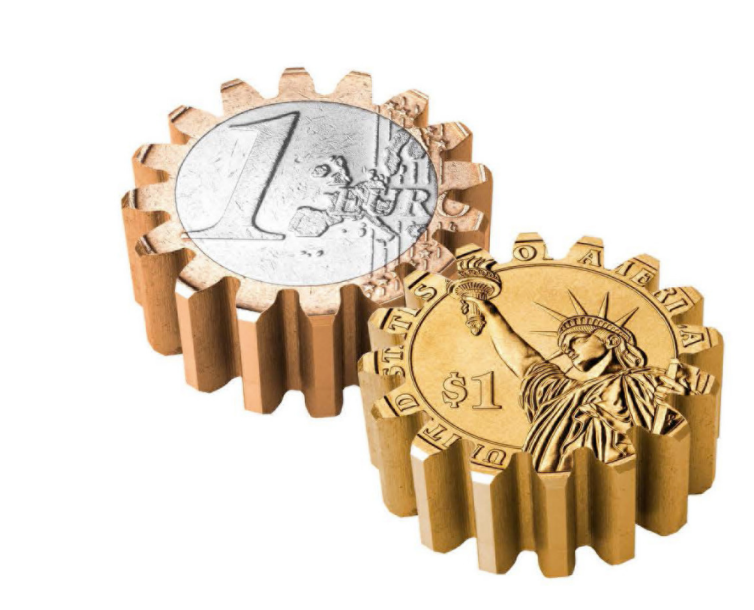
\includegraphics[width=0.9\linewidth]{Cover.png}
\end{column}

\end{columns}

% ----- Footer text (bottom-right corner) -----
\vspace*{2cm} % adjust if needed
\hfill{\large\textit{Prepared by Marcos Consuegra}}

\end{frame}


\begin{frame}{What We Will Learn}

\begin{itemize}
  \item Understand the distinction between \textbf{currency}, \textbf{money}, and their core functions in the economy.
  
  \vspace{0.2cm}
  \item Study how the \textbf{value of currency} is determined in a simple model economy.
  
  \vspace{0.2cm}
  \item Explore how \textbf{monetary and fiscal policy} interact to anchor the price level.
  
  \vspace{0.2cm}
  \item Compare two main frameworks of price determination:
  \begin{itemize}
      \item \textbf{Fiscal Theory of the Price Level (FTPL)}  
      \item \textbf{Central Bank Theory of the Price Level (CBTPL)}
  \end{itemize}
  
  \vspace{0.2cm}
  \item Assess the role of \textbf{real backing} (taxes, assets, gold) in ensuring a stable value of currency.
\end{itemize}
\end{frame}


% OUTLINE
\begin{frame}{Outline}
\tableofcontents
\end{frame}

% ======================================
\section{Currency and Money: Concepts}
% ======================================



\begin{frame}{Currency: Metallic (Commodity) Regime}

\begin{itemize}
  \item The term \textbf{currency} refers to a well-defined monetary unit issued under a recognized authority.

  \vspace{0.2cm}
  \item \textbf{Example – The Florentine Florin}  
  Struck by the Republic of Florence and circulating between \textbf{1252 and 1533}:
  \begin{itemize}
    \item A gold coin containing \textbf{54 grains} ($\approx$ 3.499 g $\approx$ 0.1125 troy oz) of fine gold.
    \item Featured a consistent alloy and purity.
    \item Bore the emblem of the city (\textit{giglio}) on one side and \textbf{Saint John the Baptist} on the reverse.
  \end{itemize}

  \vspace{0.2cm}
  \item Metallic coins had \textbf{intrinsic value}, directly linked to their precious-metal content.
\end{itemize}
\end{frame}

\begin{frame}{The Florentine Florin}
\centering
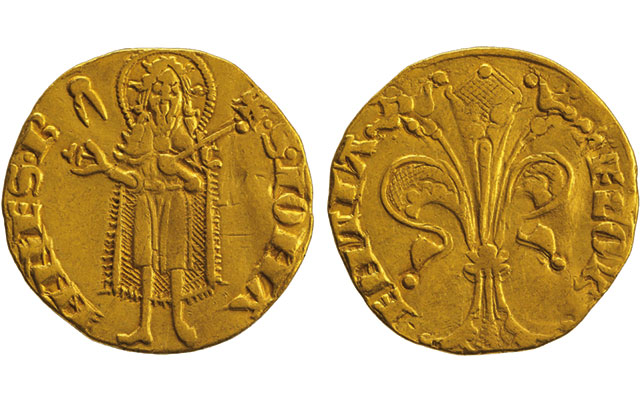
\includegraphics[width=0.65\linewidth]{Figures/FlorentinFlorin.jpg}\\[0.3cm]
{\scriptsize Florentine Florin (Republic of Florence, 13th–16th century).\\
Obverse: \textit{giglio}; Reverse: Saint John the Baptist.}
\end{frame}

\begin{frame}{Currency: Paper-Backed Regime}

\begin{itemize}
  \item \textbf{Example – The U.S. Dollar under the Gold Standard}  
  formally established by the \textbf{Gold Standard Act of 1900} and maintained until \textbf{1933}.
  \begin{itemize}
    \item Each dollar was defined as \textbf{23.22 grains of gold} ($\approx$ 1.5046 g).
    \item The dollar was a \textbf{liability of the U.S. Treasury} and an \textbf{asset for the bearer}.
    \item Gold certificates explicitly stated:  
    \textit{“This certifies that there have been deposited in the Treasury of the United States one dollar in gold coin, payable to the bearer on demand.”}
  \end{itemize}

  \vspace{0.2cm}
  \item This system linked the value of paper currency to a \textbf{fixed quantity of gold}, ensuring convertibility.
\end{itemize}
\end{frame}

\begin{frame}{U.S. Dollar under the Gold Standard}
\centering
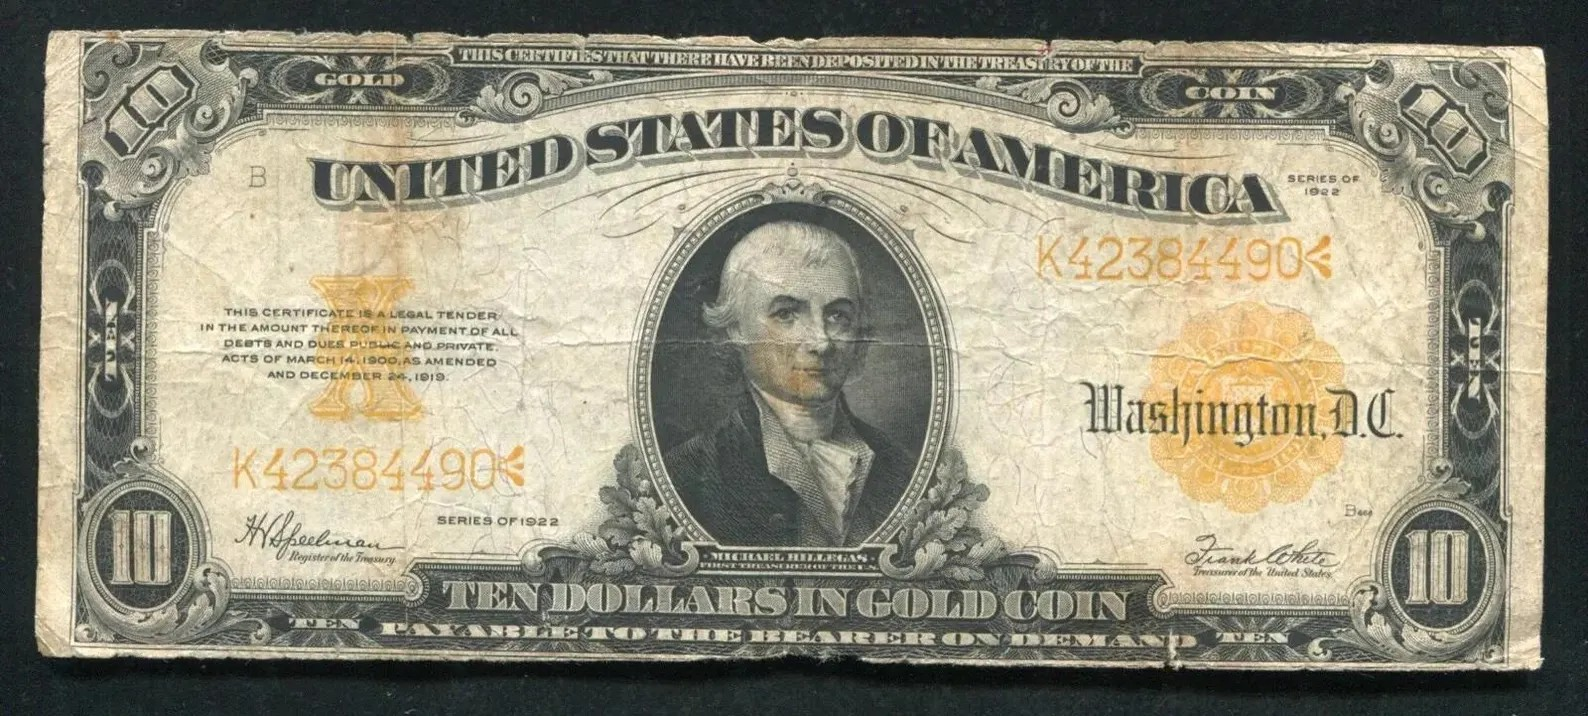
\includegraphics[width=0.7\linewidth]{Figures/GoldDollar.png}\\[0.4cm]
{\scriptsize U.S. Gold Certificate, early 20th century.\\
Printed statement: “This certifies that there have been deposited in the Treasury of the United States one dollar in gold coin, payable to the bearer on demand.”}
\end{frame}

  \begin{frame}{Intrinsically Worthless Currency}

\begin{itemize}
  \item The \emph{currency unit} is \textbf{not} tied to any commodity.
  
  \vspace{0.2cm}
  \item An \textbf{intrinsically worthless currency} is a claim that makes no other promise than to be redeemable in units of itself.
  
  \vspace{0.2cm}
  \item A dollar is simply a claim to \textbf{...another dollar!}
  
  \vspace{0.2cm}
  \item ``\$1'' represents one unit of \emph{central bank (CB) liabilities}.
  
  \vspace{0.2cm}
  \item The CB can create such liabilities \textbf{at will}, subject only to its policy objectives.
\end{itemize}
\end{frame}


\begin{frame}{U.S. Dollar Today}
\centering
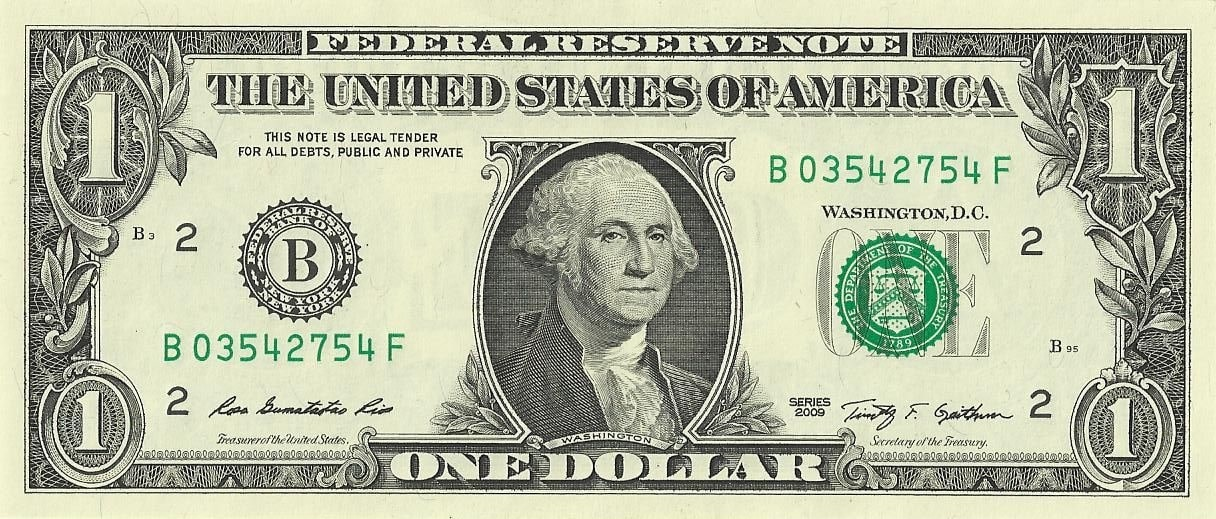
\includegraphics[width=0.7\linewidth]{Figures/Dollar.jpg}\\[0.4cm]
\end{frame}


\begin{frame}{British Pound Today}
\centering

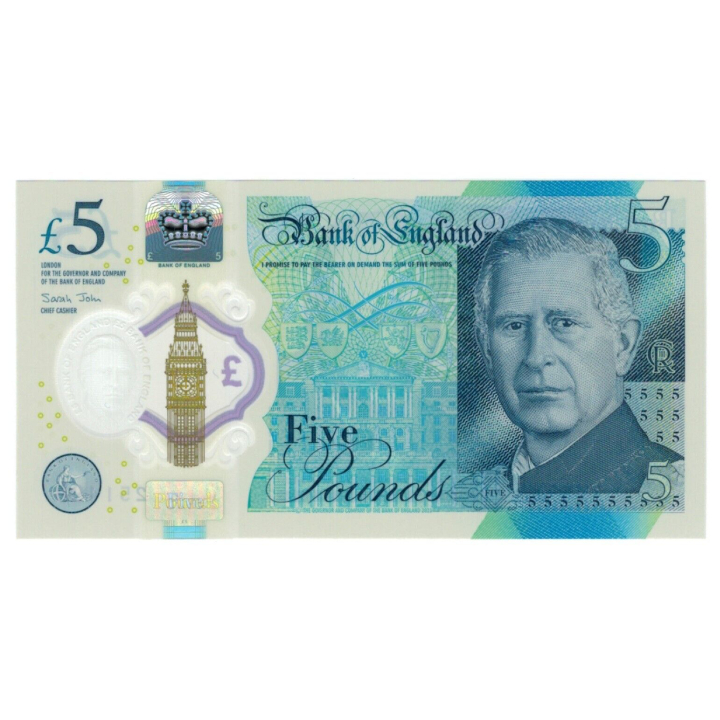
\includegraphics[height=0.78\textheight,keepaspectratio]{Figures/Pounds.jpg}\\[0.1cm]
{\scriptsize Printed statement: ``Bank of England. I promise to pay the bearer on demand the sum of five pounds.''}
\end{frame}

\begin{frame}{Three Properties of Currency}

\begin{enumerate}
  \item \textbf{Unit of account} — the numéraire for prices and contracts.
  \item \textbf{Medium of exchange} — the means of payment in transactions.
  \item \textbf{Store of value} — maintains its value across time and contingencies (i.e., keeps its promises).
\end{enumerate}

\vspace{0.6em}
\textbf{Remarks}
\begin{itemize}
  \item The \emph{unit of account} is not an essential property of currency.
  \item In medieval times, the unit of account was often an \emph{imaginary unit} that did not circulate physically.
  \item The \emph{store-of-value} property should not be confused with purchasing power:
  \begin{itemize}
      \item A gold coin guaranteed its \textbf{intrinsic metal content}, not its purchasing power.  
      \item A modern dollar banknote maintains its \textbf{nominal dollar value} over time and is a perfect store of value.
  \end{itemize}
\end{itemize}
\end{frame}

\begin{frame}{Money}

\begin{itemize}
  \item \textbf{Money} consists of claims on currency that share its key properties — being a \textbf{medium of exchange} and a \textbf{store of value} — to varying degrees.
  
  \vspace{0.3cm}
  \item \textbf{Currency is money}, but \textbf{money is not necessarily currency.}
  
  \vspace{0.3cm}
  \item A deposit at a commercial bank is not currency, but it is a \textbf{claim on currency}.  
  It functions as money because it is used as a medium of exchange and serves as a store of value — as long as the issuer (the bank) can honor redemption.  
  For the issuer, however, redeeming deposits is not as trivial as it is for the central bank.
\end{itemize}

\vspace{0.4em}
\end{frame}



% ======================================
\section{Model}
% ======================================

% -----------------------------
\begin{frame}{Model Overview}
\textbf{Economic Setting}
\begin{itemize}
  \item Infinite-horizon, closed economy with perfect foresight
  \item Single consumption good $C$ with constant endowment $Y$
\end{itemize}

\textbf{Agents}
\begin{itemize}
  \item Representative consumer
  \item Treasury
  \item Central Bank (CB)
\end{itemize}

\textbf{One Currency = CB's liabilities}
\begin{itemize}
  \item Cash $M_t$
  \item Reserves $X_t$
\end{itemize}
\end{frame}

% -----------------------------
\begin{frame}{Representative Consumer: Preferences}
\textbf{Intertemporal Utility}
\begin{equation}
\sum_{t=t_0}^{\infty} \beta^{t-t_0} \, U(C_t), 
\label{eq: utility}
\end{equation}
where $\beta$ with $0<\beta<1$ is the subjective discount factor in preferences.

\vspace{0.5cm}
\textbf{Properties of $U(C_t)$}
\begin{itemize}
  \item $U'(C_t) > 0$
  \item $U''(C_t) < 0$
\end{itemize}
\end{frame}

\begin{frame}[label=orig_budget]{Budget Constraint}

\textbf{Budget Constraint at time $t$}
\begin{equation}
\frac{B_t}{1+i_t} + \frac{X_t}{1+i_t^X} + M_t + P_t C_t + T_t
= B_{t-1} + X_{t-1} + M_{t-1} + P_t Y.
\label{eq: budget}
\end{equation}

\textbf{Where}
\begin{itemize}
  \item $B_t$: default-free one-period bond (unit face value), discounted at nominal rate $i_t$
  \item $X_t$: CB reserves, paying $i_t^X$
  \item $M_t$: cash (zero interest)
  \item $P_t$: price of consumption good
  \item $T_t$: lump-sum taxes (negative = transfers)
  \item $Y$: constant endowment of goods
\end{itemize}

\textbf{Portfolio constraints}
\begin{itemize}
  \item Bonds: $B_t$ can be held as asset $(>0)$ or issued as debt $(<0)$
  \item Cash and reserves: $M_t \ge 0$, $X_t \ge 0 \ \forall \ t \ge t_0$
\end{itemize}
\end{frame}

\begin{frame}{Transmission Mechanism of the Policy Rate}

\begin{itemize}
  \item The CB sets the interest rate on reserves, denoted by $i_t^X$.
  \item The CB supplies a positive amount of reserves: $X_t > 0$.
  \item Bonds $B_t$ and reserves $X_t$ are both default-free and have identical payoffs.
\end{itemize}

\begin{block}{No-Arbitrage Condition}
Since reserves are in \textbf{positive supply}, no-arbitrage implies that the \textbf{market} interest rate on default-free securities must equal the interest rate on reserves:
\[
i_t = i_t^X.
\]

\textbf{Key implication:} By choosing $i_t^X$—the interest rate on its liabilities, which are default-free by definition of currency—the CB effectively determines the short-term interest rate on any other default-free security.
\end{block}

\begin{itemize}
  \item From now on, $i_t$ denotes the policy rate.
\end{itemize}

\end{frame}

\begin{frame}{Cashless Equilibrium and the Zero Lower Bound}
\begin{itemize}
  \item From the budget constraint \eqref{eq: budget}, cash and bonds are \textbf{perfect substitutes} as media of exchange.
  \item Bonds pay a non-negative interest rate, while cash yields zero.
  \item It follows, when $i_t>0$, bonds dominate cash, and money demand is zero.
  \item The existence of cash implies the \textbf{zero lower bound (ZLB)}:
  \[
  i_t \ge 0.
  \]
  \item \textit{Proof by contradiction:}  
  If $i_t<0$, consumers could borrow ($B_t<0$), invest in cash, pay back debt, and earn a profit with certainty.
\end{itemize}
\end{frame}

\begin{frame}{Cashless Equilibrium and the Zero Lower Bound}
\begin{block}{Results}
\begin{enumerate}
  \item The option to hold cash sets a zero lower bound on the nominal interest rate: $i_t \geq 0$.
  \item In equilibrium:
  \[
  M_t = 0 \quad \forall\, t \ge t_0,
  \]
  unless $i_t = 0$.
\end{enumerate}
\end{block}

\begin{itemize}
  \item From now on, we assume a \textbf{cashless equilibrium}:
  \[
  M_t = 0 \quad \text{for all } t \ge t_0.
  \]
\end{itemize}
\end{frame}


\begin{frame}{Borrowing Limit}


\begin{itemize}
  \item Consumers cannot borrow indefinitely (i.e.\ hold a negative $B_{t-1}$ forever).
  \item Moreover, their debt—carrying a default-free interest rate $i_t$—must be repaid with certainty. Debt must be backed by the present discounted value (PDV) of future net surpluses. 
\end{itemize}
\noindent\textbf{Nominal borrowing limit}
\begin{equation}
\underbrace{-\,B_{t-1}}_{\text{\scriptsize debt}}
\;\le\;
\underbrace{X_{t-1}}_{\text{\scriptsize assets}}
+\;
\underbrace{\sum_{j=0}^{\infty} 
\tilde{R}_{t,t+j}\big(P_{t+j}Y_{t+j}-T_{t+j}\big)}_{\text{\scriptsize present discounted value of net income}}
\;<\;\infty,
\label{eq:nom_borrowing}
\end{equation}

\hspace{0.6cm}\textit{where} $\tilde{R}_{t,t+j}$ is the nominal discount factor from period $t+j$ with respect to time $t$:
\vspace{-0.3cm}
\[
\tilde{R}_{t,t+j}
= \prod_{i=1}^{j} \frac{1}{1 + i_{t+i-1}},
\qquad 
\tilde{R}_{t,t} \equiv 1,
\qquad 
j \ge 1.
\label{eq:nom_discount_fac}
\]
\end{frame}


\begin{frame}{Borrowing Limit in Real Terms}

\begin{itemize}
    \item The nominal borrowing limit \eqref{eq:nom_borrowing} can be expressed in real terms:
\end{itemize}

\vspace{0.25cm}
\noindent\textbf{Real borrowing limit}
\begin{equation}
  -\,\frac{B_{t-1}}{P_t} \;\le\; \frac{X_{t-1}}{P_t} 
  + \sum_{j=0}^{\infty} R_{t,t+j} \left( Y - \frac{T_{t+j}}{P_{t+j}} \right) 
  < \infty,
\label{eq:real_borrowing}
\end{equation}
\hspace{0.65cm} where $R_{t,t+j}$ is the real discount factor from $t+j$ w.r.t. time $t$.

\vspace{0.25cm}
\noindent\textbf{Real discount factor}
\[
R_{t,t+j} = \prod_{i=1}^{j} \frac{1}{1 + r_{t+i-1}}, 
\quad R_{t,t} \equiv 1, 
\quad j \ge 1.
\label{eq:real_discount_fac}
\]

\begin{itemize} \item \textbf{Note:} The real interest rate $r$ is defined as $1+r_t \equiv (1+i_t)\frac{P_t}{P_{t+1}}$. \end{itemize}

\end{frame}


\begin{frame}[label=borrowing]{Intertemporal Budget Constraint}


\begin{itemize}
  \item The borrowing limit ~(\ref{eq:real_borrowing}) is \textbf{equivalent} to the household’s intertemporal budget constraint, using the flow budget constraint (\ref{eq: budget}).
\end{itemize}

\vspace{0.25cm}
\noindent\textbf{Intertemporal Budget Constraint}
\begin{equation}
\sum_{t=t_{0}}^{\infty} R_{t_{0},t}\,C_{t}
\;\leq\;
\frac{B_{t_{0}-1}+X_{t_{0}-1}}{P_{t_{0}}}
+\sum_{t=t_{0}}^{\infty} R_{t_{0},t}\!\left(Y - \frac{T_{t}}{P_{t}}\right).
\label{eq:borrowing}
\end{equation}

\begin{itemize}
  \item The PDV of consumption cannot exceed:
  \begin{itemize}
    \item the initial real value of financial assets, and
    \item the PDV of real net income.
  \end{itemize}
\end{itemize}

\vspace{0.3cm}
\begin{center}
  \hyperlink{borrowing_proof}{\beamerbutton{See Proof in Appendix}}
\end{center}

\end{frame}

\begin{frame}[label=limit]{Asset Limit Condition}

\begin{itemize}
    \item Constraints  \eqref{eq:real_borrowing} or \eqref{eq:borrowing} can be equivalently expressed, using the flow budget constraint (\ref{eq: budget}), as an asset limit constraint.
\end{itemize}

\vspace{0.25cm}
\noindent\textbf{ Asset Limit Constraint}
\begin{equation}
\lim_{t\to \infty} \left\{ R_{t_0,t} \left( \frac{B_{t-1}+X_{t-1}}{P_t} \right) \right\} \ge 0.  \label{Blimit}
\end{equation}

\begin{itemize}
    \item This condition requires that the discounted value of the household’s asset holdings remain non-negative in the limit.
\end{itemize}

\vspace{0.3cm}
\begin{center}
\hyperlink{limit_proof}{\beamerbutton{See Proof in Appendix}}
\end{center}

\end{frame}
\begin{frame}[label=euler]{Consumer Optimality: Euler Equation}


\begin{itemize}
  \item The consumer’s intertemporal optimization problem yields the \textbf{Euler equation}.
\end{itemize}

\vspace{0.3cm}
\noindent\textbf{Euler Equation}
\begin{equation}
\underbrace{U_c(C_t)}_{\text{\scriptsize marginal utility of consumption}}
= 
\underbrace{\beta\,(1+r_t)\,U_c(C_{t+1})}_{\text{\scriptsize marginal utility of saving}},
\label{eq:euler}
\end{equation}
\hspace{0.75cm}where $U_c(C_t)$ denotes the marginal utility of consumption at time~$t$.
\vspace{0.2cm}
\begin{itemize}
  \item At the optimum, the marginal utility of consuming one unit today equals the marginal utility of saving that unit for next period.

\end{itemize}

\vspace{0.25cm}
\begin{center}
  \hyperlink{euler_proof}{\beamerbutton{See Proof in Appendix}}
\end{center}
\end{frame}

\begin{frame}{Consumer Optimality: IBC or Transversality Condition}

\begin{itemize}
    \item At the optimum, consumers exhaust all resources, i.e., the intertemporal budget constraint holds with equality:
\end{itemize}
\vspace{0.25cm}

\textbf{Intertemporal Budget Constraint}
\begin{equation}
\sum_{t=t_0}^{\infty} R_{t_0,t} C_t =
\frac{B_{t_0-1}+X_{t_0-1}}{P_{t_0}} +
\sum_{t=t_0}^{\infty} R_{t_0,t} \left( Y_t - \frac{T_t}{P_t} \right),
\label{eq: IBCCE}
\end{equation}

\vspace{0.25cm}
   \hspace{0.7cm} or, equivalently, the asset limit condition \eqref{Blimit} holds with equality:
\vspace{0.25cm}

\textbf{Transversality Condition}
\begin{equation}
\lim_{t \to \infty} R_{t_0,t} \frac{B_{t-1}+X_{t-1}}{P_t} = 0.
\label{eq: Trans}
\end{equation}

\end{frame}

\begin{frame}{Central Bank}

\begin{itemize}
    \item In this cashless economy, the CB: 
    \vspace{0.25cm}
    \begin{itemize}
        \item \textbf{issues CB reserves} $X^{C}$ (the only liability)
    \vspace{0.25cm}
    \item \textbf{holds assets} $B^{C}$, private or treasury bonds 
    \vspace{0.25cm}
    \item \textbf{makes transfers} $T^{C}$ to the treasury (positive = remittances, negative = subsidies)
    \end{itemize}
\end{itemize}

\vspace{0.5cm}
\noindent\textbf{CB Flow Budget Constraint}
\begin{equation}
\frac{B_{t}^{C}}{1+i_{t}}-\frac{X_{t}^{C}}{1+i_{t}}  \;=\; B_{t-1}^{C}-X_{t-1}^{C}- T_{t}^{C} .
\label{CBBC1}
\end{equation}

\end{frame}


\begin{frame}{Central Bank: Key Properties}

\begin{itemize}
    \item Reserves $X^{C}$ are claims on themselves; they can \textbf{always} be paid, even if $B_t^C = 0$ 
    
    $\longrightarrow$   \textbf{No} solvency condition is required on $X^{C}$. 
    \vspace{0.25cm}
    \item Given $X_{t-1}^C$, the CB can freely choose both the quantity of reserves $X_t^C$ and the interest rate $i_t$.
    \vspace{0.25cm}
    \item By choosing the transfers policy $T_t^C$, asset holdings $B_t^C$ adjust according to the flow budget constraint \eqref{CBBC1}.

\end{itemize}

\end{frame}

    \begin{frame}{Treasury Budget Constraint}
    
    \begin{itemize}
    \item The Treasury issues debt. At time $t$, it services its outstanding obligations $B_{t-1}^{F}$ using:
    \vspace{-0.2cm}
    \begin{itemize}
            \item Lump-sum taxes $T_t$ (net of transfers)
            \item CB remittances $T_t^C$
            \item Issuance of new debt $B_t^F$
        \end{itemize}
    \end{itemize}
    
    \vspace{0.25cm}
    \noindent\textbf{Treasury Budget Constraint}
    \begin{equation}
    B_{t-1}^{F} = T_t + T_t^C + \frac{B_t^F}{1+i_t}.
    \label{BudgetT}
    \end{equation}
    
    \begin{itemize}
        \item $B_{t-1}^{F}$ are claims on currency, \textbf{not} currency itself. They are not, by definition, default-free!
        \vspace{0.25cm}
        \item To be default-free, Treasury debt must satisfy a solvency constraint.
    \end{itemize}
    
    \end{frame}
    

\begin{frame}{Treasury Solvency and No-Ponzi Conditions} 

\begin{itemize}
\item Treasury debt should be repaid with certainty to be default-free (and paying the default-free rate $i$):

\begin{equation*}
\underbrace{B_{t-1}^{F}}_{\text{\scriptsize Treasury debt}}
\;\le\;
\underbrace{\sum_{j=0}^{\infty} 
\tilde{R}_{t,t+j}\,\big(T_{t+j}+T_{t+j}^{C}\big)}_{\text{\scriptsize PDV of the Treasury's resources}}
\;<\;\infty,
\end{equation*}

\noindent or in \textbf{real terms:} 
\begin{equation} \frac{B_{t-1}^{F}}{P_t} \le \sum_{j=0}^{\infty} R_{t,t+j}\,\left(\frac{T_{t+j}}{P_{t+j}} + \frac{T_{t+j}^C}{P_{t+j}}\right) < \infty, \label{DebtBB} \end{equation} 

\noindent or, equivalently, as a \textbf{no-Ponzi condition:} 
\begin{equation} \lim_{t\to\infty} R_{t_0,t} \frac{B_{t-1}^F}{P_t} \le 0. \label{Limit_Debt_T} \end{equation}
\end{itemize}

\end{frame}


\begin{frame}{Treasury - Implications for the Model}

\begin{itemize}
    \item The treasury cannot accumulate debt indefinitely; it must be covered by taxes and CB remittances in present value.
    \item If taxes are reduced in certain periods, they must increase in later periods to maintain solvency.
    \item For the subsequent analysis, we assume that condition \eqref{DebtBB} or, equivalently, \eqref{Limit_Debt_T} holds with equality.
    \item The equality assumption is supported by political-economic considerations (excessive taxation is costly) or by the rationale that the treasury does not intend to accumulate a positive long-term asset position.

\end{itemize}

\end{frame}

\begin{frame}[label=market]{Market Clearing Conditions}

\begin{itemize}
    \item Debt issued by the government ($B^F$) is held either by the CB ($B^C$) or the consumer ($B$). CB reserves ($X^C$) are held only by the consumer ($X$).
\end{itemize}

\vspace{0.25cm}
\noindent\textbf{Asset Market Clearing}
\begin{equation}
B_t^{F} = B_t^{C}+B_t,
\label{eq: Bonds}
\end{equation}
\begin{equation}
X_t^{C} = X_t.
\label{eq: reserves}
\end{equation}

\vspace{0.25cm}
\noindent\textbf{Goods Market Clearing}
\[
C_t=Y.
\]

\begin{itemize}
    \item Consumption equals output, consistent with a closed economy with no investment and no government purchases.
\end{itemize}

\vspace{0.3cm}
\begin{center}
\hyperlink{gdp_proof}{\beamerbutton{See Proof in Appendix}}
\end{center}

\end{frame}


\begin{frame}{Equilibrium Condition: Fisher Equation}
\small

\begin{itemize}
  \item In equilibrium, goods-market clearing implies
  \[
  C_t = Y.
  \]
  \item Substituting $C_t=Y$ into the Euler equation~\eqref{eq:euler} gives the Fisher equation.
\end{itemize}

\vspace{0.2cm}
\noindent\textbf{Fisher Equation}
\begin{equation}
\underbrace{1+i_t}_{\text{\scriptsize gross nominal interest rate}}
\;=\;
\underbrace{\frac{1}{\beta}}_{\text{\scriptsize gross real interest rate}}
\;\underbrace{\frac{P_{t+1}}{P_t}}_{\text{\scriptsize gross inflation}},
\label{eq: Fisher}
\end{equation}

\begin{itemize}
  \item This condition links the nominal interest rate to the real interest rate and expected inflation.
  \item Since the endowment is constant, the gross real interest rate is constant and equal to $1/\beta$.
\end{itemize}

\end{frame}

\begin{frame}{Equilibrium Condition: Intertemporal Resource Constraint}
\small

\begin{itemize}
  \item Using $C_t=Y$ together with the Fisher equation~\eqref{eq: Fisher}, the household intertemporal budget constraint~\eqref{eq: IBCCE} becomes:
\end{itemize}

\vspace{0.2cm}
\noindent\textbf{Intertemporal Resource Constraint}
\begin{equation}
\frac{B_{t_0-1}+X_{t_0-1}}{P_{t_0}}
=
\sum_{t=t_0}^{\infty}\beta^{\,t-t_0}\frac{T_t}{P_t}.
\label{eq: IBCTT}
\end{equation}

\begin{itemize}
  \item \textbf{Left-hand side:} the real value of government liabilities held by the private sector at time $t_0$.
  \item \textbf{Right-hand side:} the present discounted value of real taxes.
  \item This is \textbf{not} a solvency condition for the government as a whole; it is an \textbf{equilibrium condition}.
\end{itemize}

\end{frame}



\begin{frame}{Equilibrium Condition: Treasury Solvency}
\small

\begin{itemize}
  \item The Treasury, unlike the central bank, cannot issue claims that are redeemable in units of themselves.
  \item Therefore, Treasury debt must satisfy its own solvency condition.
  \item Using~\eqref{DebtBB} with equality and the Fisher equation~\eqref{eq: Fisher}, we obtain:
\end{itemize}

\vspace{0.2cm}
\noindent\textbf{Treasury Solvency Condition}
\begin{equation}
\frac{B_{t_0-1}^{F}}{P_{t_0}}
=
\sum_{t=t_0}^{\infty}\beta^{\,t-t_0}
\left(\frac{T_t}{P_t}+\frac{T_t^{C}}{P_t}\right).
\label{eq: TreasurySolvency}
\end{equation}

\begin{itemize}
  \item Treasury solvency requires the real value of outstanding debt to be backed by the present discounted value of real taxes and CB remittances.
\end{itemize}

\end{frame}

\begin{frame}{Equilibrium Conditions: Government Budget Constraints}
\small

\begin{itemize}
  \item In equilibrium, the central bank and the Treasury must satisfy their respective flow budget constraints period by period.
\end{itemize}

\vspace{0.2cm}
\noindent\textbf{Central Bank Budget Constraint}
\begin{equation}
\frac{X_t-B_t^{C}}{1+i_t}
=
X_{t-1}-B_{t-1}^{C}+T_t^{C}.
\label{eq: FlowG}
\end{equation}

\vspace{0.3cm}
\noindent\textbf{Treasury Budget Constraint}
\begin{equation}
\frac{B_t^{F}}{1+i_t}
=
B_{t-1}^{F}-T_t-T_t^{C}.
\label{eq: TBC}
\end{equation}

\begin{itemize}
  \item These equations describe how liabilities, assets, taxes, and remittances evolve over time.
\end{itemize}

\end{frame}

\begin{frame}{Competitive Equilibrium: Definition}
\small

Given initial conditions $B_{t_0-1}^{C}, B_{t_0-1}^{F}, X_{t_0-1}$, a \textbf{competitive equilibrium} is a set of sequences
\[
\{P_t,i_t,X_t,B_t^{C},T_t^{C},B_t^{F},T_t,B_t\}_{t=t_0}^{\infty},
\]
with
\[
\{P_t,i_t,X_t,B_t^{C}\}_{t=t_0}^{\infty}\ge 0,
\]
such that:

\vspace{0.1cm}
\begin{enumerate}
  \item households optimize;
  \item the Fisher equation \eqref{eq: Fisher}, the intertemporal resource constraint \eqref{eq: IBCTT}, and the government budget constraints \eqref{eq: FlowG}--\eqref{eq: TBC} hold;
  \item markets clear:
  \[
  B_t^{F}=B_t^{C}+B_t,\qquad X_t^{C}=X_t,\qquad C_t=Y;
  \]
  \item the tax sequence $\{T_t\}_{t=t_0}^{\infty}$ satisfies Treasury solvency \eqref{eq: TreasurySolvency}, at each point in time, given that Treasury's debt follows (\ref{eq: TBC}).

\end{enumerate}

\end{frame}


\begin{frame}{Government Policy and Degrees of Freedom}
\small

\begin{itemize}
  \item The equilibrium characterization reveals \textbf{four policy degrees of freedom}.
  
  \vspace{0.2cm}
  \item The central bank can choose the sequences
  \[
  \{i_t,\;X_t,\;T_t^{C}\}_{t=t_0}^{\infty},
  \]
  while its asset holdings adjust through~\eqref{eq: FlowG}.
  
  \vspace{0.2cm}
  \item Given the paths of prices and CB remittances, the Treasury chooses the tax sequence
  \[
  \{T_t\}_{t=t_0}^{\infty}
  \]
  that satisfies the solvency condition~\eqref{eq: TreasurySolvency}.
\end{itemize}

\vspace{0.2cm}
\textbf{Implication:}  
Without a fully specified monetary and fiscal policy, the model does not determine a unique equilibrium price level.

\end{frame}


\begin{frame}{Monetary Policy Insights}
\textbf{Key Insights:}
\begin{itemize}
    \item The economy does not have an inherent tendency to select a unique price level without the CB specifying policy sequences $\{i_t, X_t, T_t^C\}_{t=t_0}^\infty$.
    \vspace{0.3cm}
    \item Forward guidance is important: policymakers must communicate both current and future paths of policy to eventually be able to determine equilibrium.
    \vspace{0.3cm}
    \item Balance-sheet policies matter: specifying interest rates alone is not sufficient to uniquely determine the price level (as shown next).
\end{itemize}
\end{frame}

% ======================================
\section{Determining the Value of the Currency}
% ======================================

\begin{frame}{Value of the Currency: Limits of Interest-Rate Policy}
\begin{itemize}
    \item We show that interest-rate policy alone cannot determine the currency's value.
    \item Using the Fisher equation (\ref{eq: Fisher}), if the CB pegs $i_t = i$, only the rate of price changes is determined, i.e. $\frac{P_{t+1}}{P_{t}}$, not the price level itself.
    \item This indeterminacy result also holds with active policies reacting to deviations from a target $\bar{P}$ as the following:
\end{itemize}
\textbf{Policy Rule}
    \begin{equation} \label{eq: int_rule}
        1 + i_t = \max \left\{ \frac{1}{\beta} \left( \frac{P_t}{\bar{P}} \right)^\phi, 1 \right\}, \quad \phi \ge 0.
    \end{equation}
\begin{itemize}
    \item In \eqref{eq: int_rule}, the interest rate is equal to the real rate $1/\beta$ and reacts with a coefficient $\phi$ to the ratio of the current price level with respect to the target $\bar{P}$, unless the zero lower bound binds.
\end{itemize}
\end{frame}

\begin{frame}{Price-Level Indeterminacy}
\begin{itemize}
    \item Combining the Fisher equation (\ref{eq: Fisher}) and the interest-rate rule \eqref{eq: int_rule} gives a non-linear difference equation for the price level:
    \begin{equation} \label{eq: price_level_rule}
        \frac{P_{t+1}}{P_t} = \max \left\{ \left(\frac{P_t}{\bar{P}} \right)^\phi, \beta \right\}.
    \end{equation}
    \item For $\phi > 0$, infinite solutions exist, all indexed by $P_{t_0} \in (0,\infty)$ :
    \begin{itemize}
        \item Stationary solution exists only if $P_{t_0} = \bar{P}$
        \item $P_{t_0} > \bar{P} \Rightarrow $  inflationary path;  
        $P_{t_0} < \bar{P}\Rightarrow $  deflationary path
        \end{itemize}
    \item For $\phi = 0$, infinite stationary solutions exist, all indexed by $P_{t_0} \in (0,\infty)$
    \item \textbf{Conclusion:} Interest-rate rules, even Taylor-type rules, cannot uniquely determine the price level without specifying appropriately additional policy instruments (\textit{the other degrees of freedom}).
\end{itemize}
\end{frame}

\begin{frame}{Phase Diagram Illustration}
\centering
% Include the figure if it exists, otherwise display placeholder text
\IfFileExists{Figures/Figure2.png}{%
    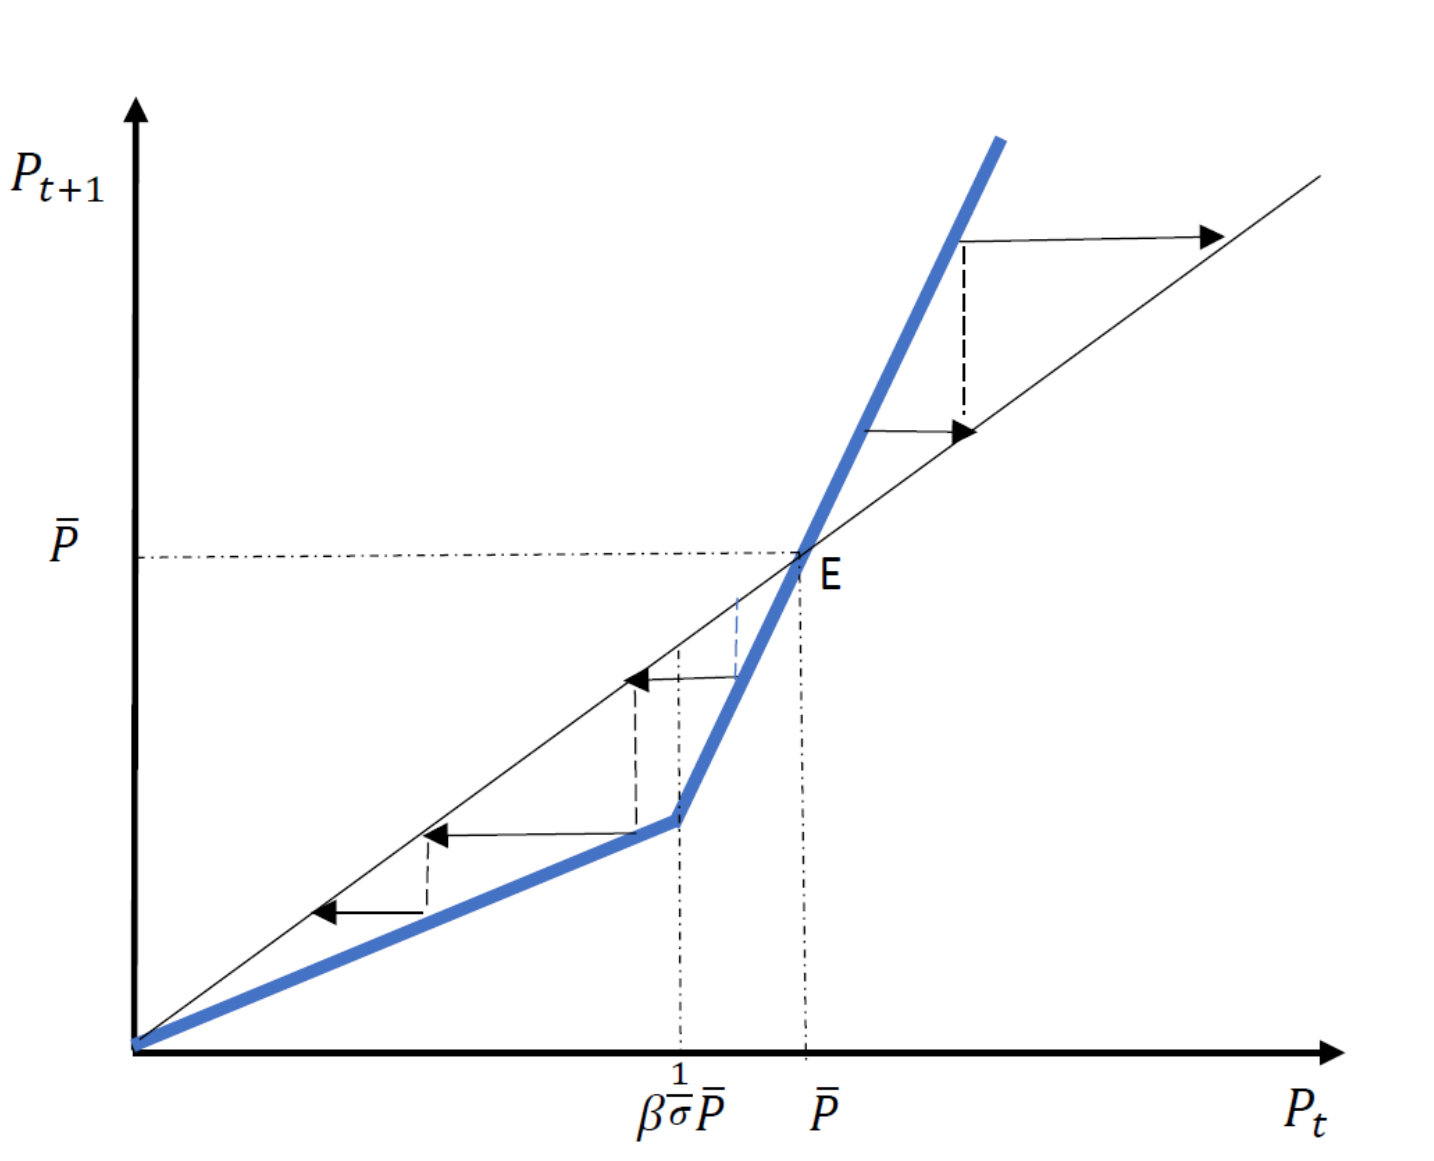
\includegraphics[height=0.7\textheight,keepaspectratio]{Figures/Figure2.png}%
}{%
    \textit{(Insert Figure2.png here)}%
}

\vspace{0.5em}


Phase diagram for $\phi>0$. The stationary solution is $P_t=\bar P$. 

If $P_t \le \beta^{1/\phi}\bar P$, the deflation rate is $\beta$ (with $0<\beta<1$).
\end{frame}

% ======================================
\section{Fiscal Theory of the Price Level}
% ======================================

\begin{frame}{Fiscal Theory of the Price Level (FTPL) – Concept}
\begin{itemize}
    \item FTPL critically relies on the \textbf{coordination} between monetary and fiscal policy.

    \item \textbf{Distinction between Treasury and CB liabilities:}
  \begin{itemize}
    \item \textbf{Treasury debt} promises payment in a currency for which the Treasury has \textbf{limited resources}.
    \item \textbf{CB liabilities} are redeemable in \textbf{units of themselves}, and can therefore be issued in \textbf{unlimited supply}.
  \end{itemize}
    \vspace{0.15cm}    
    \item In FTPL the CB \textbf{fully guarantees} treasury debt. Therefore, the solvency condition \eqref{DebtBB} no longer constraints the path of taxes.
    \vspace{0.15cm}
    \item The government budget constraints can be now consolidated, by using \eqref{CBBC1}, \eqref{BudgetT} and bond market clearing \eqref{eq: Bonds}:
    \end{itemize}
\textbf{Consolidated Government Budget Constraint}
    \begin{equation} \label{eq: gov_budget}
        \frac{B_t + X_t}{1+i_t} = B_{t-1} + X_{t-1} - T_t.
    \end{equation}
\end{frame}

\begin{frame}{Equilibrium under FTPL}


Given that tax policy is no longer constrained by solvency condition \eqref{eq: TreasurySolvency}, equilibrium is characterized by a set of sequences:
\[
\{ i_t, P_t, X_t, T_t, B_t \}_{t=t_0}^\infty,
\]
with $\{P_t, i_t, X_t \}_{t=t_0}^\infty \geq 0$ that satisfies:
\begin{itemize}
  \item Euler Equation (\ref{eq: Fisher})
  \item Intertemporal resource constaint (\ref{eq: IBCTT})
  \item Interest-rate rule (\ref{eq: int_rule})
  \item Consolidated government budget constraint (\ref{eq: gov_budget})
\end{itemize}

given initial conditions $X_{t_0-1}, B_{t_0-1}$.  
\vspace{0.3cm}
\break
Two policy instruments must be specified in addition to the interest rate:
\begin{itemize}
  \item The sequence of taxes $\{T_t\}_{t=t_0}^\infty$
  \item The sequence of reserves $\{X_t\}_{t=t_0}^\infty$, taken as arbitrary positive.
\end{itemize}

\end{frame}

\begin{frame}{Constant Real Tax Policy}
\begin{itemize}
    \item Inspecting the intertemporal resource constraint (\ref{eq: IBCTT}), the key determinant of the price level is the formulation of a tax policy.
    \vspace{0.25cm}
\item Consider the constant real tax policy:
    \begin{equation} \label{tax_policy}
    \frac{T_t}{P_t} = (1-\beta)\tau, \quad \tau>0.        
    \end{equation}
    \vspace{0.25cm}
    \item Substituting into the intertemporal budget condition (\ref{eq: IBCTT}) implies:
    \begin{equation} \label{Price_Level}
     P_{t_0} = \frac{B_{t_0-1} + X_{t_0-1}}{\tau}.
    \end{equation}
\end{itemize}
\end{frame}

\begin{frame}{Price Level Determination}
\begin{itemize}
    \item Equation \eqref{Price_Level} pins down the initial price level which implies a proportional relationship between government net liabilities and the price level.
    \vspace{0.25cm}
    
    \item The entire path $\{P_t\}_{t>t_0}^\infty$ is then uniquely determined by \eqref{eq: price_level_rule}, given $P_{t_0}$.
    \vspace{0.5cm}
\item This type of policy is called \textbf{active} because taxes are fixed in real terms and do not adjust to ensure solvency. Indeed, solvency is \textbf{guaranteed} by the CB.
\end{itemize}

\end{frame}

\begin{frame}{Tax Policy and Equilibrium Selection}
\begin{itemize}
    \item Among multiple possible paths from \eqref{eq: price_level_rule} given \eqref{eq: int_rule}, tax policy can select the equilibrium one.
    \item Define
    \[
    \tau^* = \frac{B_{t_0-1} + X_{t_0-1}}{\bar P}.
    \]
    \item Cases:
    \begin{enumerate}
        \item $\tau = \tau^* \;\Rightarrow\; P_{t_0} = \bar P$ (stationary equilibrium)
        \item $\tau > \tau^* \;\Rightarrow\; P_{t_0} < \bar P$ (deflationary path if $\phi > 0$)
        \item $\tau < \tau^* \;\Rightarrow\; P_{t_0} > \bar P$ (inflationary path)
    \end{enumerate}
    \item \textbf{Conclusion:} Under FTPL, tax policy can uniquely anchor the price level.
\end{itemize}
\end{frame}

\begin{frame}{Role of the Central Bank in the FTPL}

\begin{itemize}

  \item \textbf{CB backing:}  
  Solvency is no longer a constraint for the Treasury once the CB guarantees its debt.

  \item \textbf{Example:}  
  Substituting the tax policy~\eqref{tax_policy} into the solvency condition~\eqref{DebtBB},  
  and assuming $T_t^{C} = 0$ for all $t$, solvency requires:
  \begin{equation}
    \frac{B^{F}_{t_0-1}}{P_{t_0}} \;\leq\; \tau.
    \label{Eq:Example}
  \end{equation}

  \begin{itemize}
    \item If the equilibrium price level $P_{t_0}$ is too low relative to debt obligations  
    (i.e.\ the LHS of~\eqref{Eq:Example} $> \tau$), the Treasury is \textbf{insolvent} without the backing of the CB.
    \item To restore solvency, the Treasury would need to raise taxes ($\tau$), and change its tax policy.
  \end{itemize}

  \item \textbf{Implication:}  
  Fiscal policy can determine the price level only if the CB fully backs the Treasury’s debt.

  \item \textbf{Open question:}  
  Why should the CB back the Treasury and allow it to influence the price level?

\end{itemize}
\end{frame}


% ======================================
\section{Central Bank Theory of the Price Level}
% ======================================

\begin{frame}{Central Bank Theory of the Price Level (CBTPL) – Concept}

\begin{itemize}

  \item Unlike the FTPL, the CBTPL relies on the CB to \textbf{independently determine the price level}.

  \vspace{0.25cm}
  \item \textbf{Key practical cases:}
  \begin{itemize}
    \item Private currencies with no connection to the government.
    \item The European Monetary Union (EMU): Treasuries and the CB are separate; 
    solvency constraints for Treasuries are binding (at least before the 2011 sovereign debt crisis).
  \end{itemize}

  \vspace{0.25cm}
  \item Without CB backing, the Treasury must satisfy the solvency condition~\eqref{DebtBB}.  
  Assuming equality in~\eqref{DebtBB} and substituting into the intertemporal resource constraint~\eqref{eq: IBCTT} yields:
  \begin{equation}
    \sum_{t=t_{0}}^{\infty} \beta^{t-t_{0}}\,\frac{T_t^C}{P_t}
    \;=\;
    \frac{B_{t_0-1}^C - X_{t_0-1}}{P_{t_0}}.
    \label{eq:IBCCB}
  \end{equation}

\end{itemize}
\end{frame}

\begin{frame}{Equilibrium under CBTPL}

\textbf{Equilibrium under CBTPL:}  
An equilibrium is a set of sequences:
\[
\{ i_t, P_t, X_t, B_t^C, T_t^C \}_{t=t_0}^\infty,
\]
with $\{P_t, i_t, X_t \}_{t=t_0}^\infty \geq 0$, satisfying:
\begin{itemize}
  \item Euler equation (\ref{eq: Fisher})
  \item Interest-rate policy (\ref{eq: int_rule})
  \item CB flow budget constraint (\ref{CBBC1})
  \item Intertemporal resource constraint (\ref{eq:IBCCB})
\end{itemize}

given initial conditions $B_{t_0-1}^C, X_{t_0-1}$.  
\break

Two policy instruments must be specified by the CB in addition to the interest rate:
\begin{itemize}
  \item Sequence of reserves $\{X_t\}_{t=t_0}^\infty$, taken as arbitrary positive
  \item Sequence of non-negative remittances $\{T_t^C\}_{t=t_0}^\infty$ (to prevent treasury support)
\end{itemize}

\end{frame}

% ======================================
\begin{frame}{Discussion of the Intertemporal Resource Constraint}
\begin{itemize}
    \item The equilibrium condition \eqref{eq:IBCCB} deserves further discussion.
    \vspace{0.25cm}
    \item The present discounted value of CB remittances in \textit{equilibrium} equals the real net assets of the CB.
\vspace{0.25cm}
\item This is \textbf{not} a solvency condition, since nominal liabilities are always paid.
\vspace{0.25cm}
\item It is an equilibrium (intertemporal) resource constraint.

\vspace{0.25cm}
\item The CB can determine the initial price level with an appropriate transfer policy.

\vspace{0.25cm}
\item The intertemporal resource constraint holds because prices adjust to the chosen remittance policy, not because the CB actively adjusts remittances.

\end{itemize}
\end{frame}

\begin{frame}{Real Transfer Policy}
\begin{itemize}
    \item Consider a real transfer policy (i.e. a commitment to a sequence of remittances indexed to the price level) : $T_t^C / P_t = (1-\beta) \tau^C$, $\tau^C>0$.
    \vspace{0.25cm}
    \item Substituting into \eqref{eq:IBCCB} determines the initial price level:
    \begin{equation} \label{PdetC}
        P_{t_0} = \frac{B_{t_0-1}^C - X_{t_0-1}}{\tau^C}.
    \end{equation}
    \vspace{0.25cm}
    \item $P_{t_0}$ is positive if $B_{t_0-1}^C > X_{t_0-1}^C$, i.e., CB starts with positive net worth.
    \item Setting $\tau^C = (B_{t_0-1}^C - X_{t_0-1}) / \bar P$ pins $P_{t_0} = \bar P$, independently of $\phi$ in (\ref{eq: int_rule}).
    \vspace{0.25cm}
    \item Unlike FTPL, determination of the price level does not require cooperation between fiscal and monetary authorities.
\end{itemize}
\end{frame}

\begin{frame}{CBTPL: Net Worth and Key Equation}


\begin{itemize}
  \item The equilibrium condition~\eqref{eq:IBCCB} helps illustrate the intuition 
  behind the \textbf{price determination}.
  
  \vspace{0.25cm}
  \item \textbf{Define CB net worth:}
  \begin{equation}
  N_t^C = \frac{B_t^C - X_t}{1+i_t}.
    \label{eq: NW}
    \end{equation}
   
  
  \vspace{0.25cm}
  \item Rewriting~\eqref{eq:IBCCB} yields:
  \begin{equation}
  \underbrace{\frac{1}{P_{t_0}}(1+i_{t_0-1})\,N_{t_0-1}^C}_{\text{\scriptsize real value of CB equity}}
  \;=\;
  \underbrace{\sum_{t=t_0}^{\infty} \beta^{t-t_0}\,\frac{T_t^C}{P_t}.}_{\text{\scriptsize PDV of real remittances}}
  \label{KeyN}
  \end{equation}
  
  \vspace{0.15cm}
  \item The term $\tfrac{1}{P_{t_0}}$ represents the \textbf{price of CB equity} in units of goods.
\end{itemize}

\end{frame}


\begin{frame}{CBTPL: Interpretation and Policy Requirements}


\begin{itemize}
  \item Equation~\eqref{KeyN} highlights the link between the CB’s balance sheet 
  and the determination of the price level.

  \vspace{0.3cm}
  \item Two key requirements for \textbf{price-level determination:}
  \begin{itemize}
    \item The CB must receive an initial \textbf{transfer} at time $t_0$ 
    (from the Treasury or the private sector) to ensure positive net worth.
    \item The CB must hold \textbf{default-free securities} (e.g., $B^C$) 
    to back its liabilities.
  \end{itemize}

  \vspace{0.3cm}
  \item Intuition:  
  The value of money, hence the price level, is tied to the \textbf{real backing} 
  of the CB’s equity and the expected flow of future remittances.
\end{itemize}

\end{frame}


\begin{frame}{Requirement 1 -- Initial Transfer}
\begin{itemize}
    \item The CB cannot build net worth on its own $\rightarrow$ it must receive an initial transfer to ensure an initial positive net worth.
    \vspace{0.25cm}
    \item Rewriting the CB's budget constraint \eqref{CBBC1} using the definition of net worth, $N_t^C$, through \eqref{eq: NW}:
    \[
    N_t^C = N_{t-1}^C + \Psi_t^C - T_t^C, 
     \quad \text{with} \quad \Psi_t^C = i_{t-1} N_{t-1}^C.
    \]
    \vspace{0.25cm}
    \item If $N_{t-1}^C = 0$, then profits $\Psi_t^C = 0$ for all $t$ and $N_{t}$ cannot be positive.
    \vspace{0.25cm}
    \item  An initial transfer (real or nominal) from the Treasury or private sector is required to give the CB positive equity.
    \vspace{0.25cm}
    \item Remark: 
    This requirement can be relaxed in models where the CB holds gold or collects seigniorage.
\end{itemize}
\end{frame}

\begin{frame}{Requirement 2 – Default-Free Securities}


\begin{itemize}
  \item Equation~\eqref{PdetC} shows that \textbf{price determination depends on the presence of default-free assets} in the CB’s portfolio.

  \vspace{0.25cm}
  \item These assets must \textbf{exceed the value of liabilities} to ensure positive net worth and to generate profits.

  \vspace{0.25cm}
  \item Holding \textbf{default-free nominal securities} is essential for maintaining price-level control.
\end{itemize}

\end{frame}

\begin{frame}{Implications}


\begin{itemize}
  \item A \textbf{paper currency} requires a form of \textbf{real backing}.
  
  \vspace{0.2cm}
  \item With \textbf{governmental coordination}, such backing can be achieved through the power of \textbf{real taxes} imposed by the Treasury.
  
  \vspace{0.2cm}
  \item Without coordination, the CB can provide real backing through a policy of distributing real earnings, which requires:
  \begin{itemize}
    \item an \textbf{initial transfer} to ensure positive net worth, and  
    \item holding \textbf{default-free securities} to generate profits.  
  \end{itemize}
  
  \vspace{0.2cm}
  \item The \textbf{CBTPL} therefore shows how the CB alone can \textbf{anchor the price level}, provided it starts with \textbf{a positive net worth}.
\end{itemize}

\end{frame}


\begin{frame}{Example: Nominal Remittances Policy}
\begin{itemize}
    \item Considering a nominal remittances policy:
    \[
      T_t^C = (1-\beta)\,(B_{t_0-1}^C - X_{t_0-1}^C), \quad B_{t_0-1}^C > X_{t_0-1}^C.
    \]
    \vspace{0.15cm}
    \item Substituting again into \eqref{eq:IBCCB} yields:
    \begin{equation} \label{eq: nominal remittancy}
      (1-\beta)\sum_{t=t_0}^\infty \beta^{t-t_0}\frac{1}{P_t} \;=\; \frac{1}{P_{t_0}}.
    \end{equation}
    \vspace{0.15cm}
    \item Considering interest-rate policy \eqref{eq: int_rule}:
    \begin{itemize}
        \item \textbf{Case 1:} Pure pegging ($\phi=0$) $\;\Rightarrow\;$ no determination of $P_{t_0}$.  
        \item \textbf{Case 2:} Active policy ($\phi>0$) $\;\Rightarrow\;$ two equilibria: 1) $P_t=\bar P$ and 2) $P_t=+\infty$.  
    \end{itemize}
\end{itemize}
\end{frame}

\begin{frame}{Implications}
\begin{itemize}
    \item With a nominal remittances policy:
    \vspace{0.15cm}
    \begin{itemize}
        \item An active interest-rate policy may be necessary to pin down the price level.
       \vspace{0.25cm} 
       \item A non-monetary equilibrium exists in \eqref{eq: nominal remittancy}: $P_t = +\infty$, where the currency is worthless.
    \end{itemize}
    \item This contrasts with a real remittances policy, which uniquely determines the initial price level via CB net worth.
       \vspace{0.25cm} 
    \item Nominal transfer policies alone do not guarantee a unique price level (same under the FTPL).
         \vspace{0.25cm} 
    \item However, allowing the CB to trade in gold can remove the non-monetary equilibrium and uniquely determine prices without relying on Treasury transfers.
\end{itemize}
\end{frame}

% ======================================
\section{A Model with Gold Holdings}
% ======================================

\begin{frame}{A Model with Gold Holdings}
\begin{itemize}
    \item Extend the previous framework to include a durable commodity, \textbf{gold}.
    \vspace{0.2cm}
    \item Consumers derive utility from gold, which also forms part of the CB's assets.
    \vspace{0.2cm}
    \item Gold management allows the CB to control the price level even:
    \begin{itemize}
        \item under a nominal remittances policy, and
        \item with periods of negative net worth.
    \end{itemize}
    \vspace{0.2cm}
    \item Full convertibility into gold is \textbf{not required}, unlike a Gold Standard (see Chapter 2).
\end{itemize}
\end{frame}

\begin{frame}{Representative Consumer: Preferences with Gold}
\textbf{Intertemporal Utility}
\begin{equation}
\sum_{t=t_0}^{\infty} \beta^{t-t_0} \big[ U(C_t) + Z(g_t) \big],
\label{eq: utility_gold}
\end{equation}
where $g_t$ represents the households gold holdings providing utility.

\vspace{0.3cm}
\textbf{Properties}
\begin{itemize}
  \item $U'(C_t) > 0$, $U''(C_t) < 0$ 
  \item $Z'(g_t) > 0$, $Z''(g_t) < 0$
\end{itemize}
\end{frame}

\begin{frame}{Household Budget Constraint with Gold}
\textbf{Budget Constraint at time $t$}
\begin{equation} \label{eq: budget_gold}
\frac{B_t + X_t}{1+i_t} + P_{g,t} g_t + P_t C_t + T_t
= B_{t-1} + X_{t-1} + P_{g,t} g_{t-1} + P_t Y + P_{g,t} (g_t^S - g_{t-1}^S),
\end{equation}
\vspace{0.2cm}
where
\begin{itemize}
  \item $P_{g,t}$: price of gold in units of currency
  \item $g_t^S$: total gold in the economy owned by the households
  \item Other variables are defined as in \hyperlink{orig_budget}{\beamerbutton{Budget Constraint}}
\end{itemize}
\end{frame}

\begin{frame}{Optimal Demand of Gold}
\begin{itemize}
  \item Optimality condition with respect to gold holdings implies that:

\begin{equation} \label{eq: FOC_gold}
\frac{P_{g,t}}{P_t} = \frac{Z_g(g_t)}{U_c(C_t)} + \frac{1}{1+r_t} \frac{P_{g,t+1}}{P_{t+1}},
\end{equation}

where $Z_g(\cdot)$ is the derivative of $Z(\cdot)$ with respect to gold holdings $g_t$.
\vspace{0.3cm}
  \item The real price of gold equals the marginal rate of substitution between gold and consumption plus the discounted future real price.
\end{itemize}
\end{frame}

\begin{frame}{Intertemporal Budget Constraint with Gold}
\textbf{Intertemporal Budget Constraint with Gold}
\begin{equation} \label{eq: IBC_gold}
\sum_{t=t_0}^{\infty} R_{t_0,t} C_t = \frac{\mathcal{W}_{t_0}}{P_{t_0}} + 
\sum_{t=t_0}^{\infty} R_{t_0,t} \Bigg\{ \Big(Y - \frac{T_t}{P_t}\Big) + \frac{Z_g(g_t)}{U_c(C_t)} (g_t^S - g_t) \Bigg\}.
\end{equation}
\vspace{0.15cm}

\textbf{Initial Wealth}
\begin{equation}
\mathcal{W}_{t_0} \equiv B_{t_0-1} + X_{t_0-1} + P_{g,t_0} (g_{t_0-1} - g_{t_0-1}^S).
\end{equation}
\vspace{0.3cm}
\begin{itemize}
    \item The last term on the RHS of \eqref{eq: IBC_gold} represents the gains that the household gets by selling its gold holdings.
\end{itemize}
\end{frame}

\begin{frame}{Additional Equilibrium Conditions}
\begin{itemize}
    \item CB budget constraint with gold holdings:
    \begin{equation}
    \frac{B_{t}^{C}-X_{t}}{1+i_{t}} + P_{g,t} g_{t}^{C} =
    B_{t-1}^{C}-X_{t-1} + P_{g,t} g_{t-1}^{C} - T_{t}^{C}.
    \label{BC_gold}
    \end{equation}
    \vspace{0.2cm}
    \item For simplicity, assume a constant gold endowment, $g^S$.
     \vspace{0.2cm}
    \item Gold market equilibrium condition:
    \begin{equation}
        g^S = g_t + g_t^C,
    \end{equation}
    where $g_t^C$ are the CB’s gold holdings and $g_t$ are households’ gold holdings.
\end{itemize}
\end{frame}

\begin{frame}{CBTPL in an Economy with Gold}

\begin{itemize}
\item Consider the case in which the CB does not back the treasury.
    \item Starting from the interest-rate rule (\ref{eq: int_rule}) and equilibrium in goods, asset, and gold markets, together with the treasury solvency condition (\ref{eq: TreasurySolvency}) and $R_{t_0,t} = \beta^{t-t_0}$, we obtain using \eqref{eq: IBC_gold}:
\end{itemize}

\begin{equation}
\frac{B_{t_0-1}^{C}+P_{g,t_0} g_{t_0-1}^{C}-X_{t_0-1}}{P_{t_0}} =
\sum_{t=t_0}^{\infty} \beta^{t-t_0} \frac{Z_g(g_t)}{U_c(Y)} g_t^C +
\sum_{t=t_0}^{\infty} \beta^{t-t_0} \frac{T_t^C}{P_t}. 
\label{IBC_Gold1}
\end{equation}

\begin{itemize}
    \item \textbf{LHS}: Real net assets of the CB including gold holdings.  
    \item \textbf{RHS}: Present discounted costs of holding gold and real remittances.  
    \item Holding gold is costly (lower return than reserves since it provides utility to households).  
    \item Note: If $g_t^C = 0$ $\forall t \ge t_0$, \eqref{IBC_Gold1} reduces to \eqref{eq:IBCCB}.
\end{itemize}
\end{frame}

\begin{frame}{CBTPL in an Economy with Gold}
\begin{itemize}
    \item Define:
    \begin{equation} \label{gold_term}
        \mathcal{G}_{t_0-1} = \sum_{t=t_0}^{\infty} \beta^{t-t_0} 
        \frac{Z_g(g^S - g_t^C)}{U_c(Y)} \,(g_{t_0-1}^C - g_t^C).
    \end{equation}

    \item Using \eqref{eq: FOC_gold} and \eqref{gold_term} in \eqref{IBC_Gold1}, we can rewrite the CB intertemporal resource constrain as:
    \begin{equation}
        \frac{B_{t_0-1}^C - X_{t_0-1}}{P_{t_0}} + \mathcal{G}_{t_0-1} =
        \sum_{t=t_0}^{\infty} \beta^{t-t_0} \frac{T_t^C}{P_t} .
        \label{IBC_Gold2}
    \end{equation}

    \item Comparison with \eqref{eq:IBCCB}:
    \begin{itemize}
        \item $\mathcal{G}_{t_0-1}$ is independent of $P_{t_0}$ and given $\mathcal{G}_{t_0-1} \neq 0$ prevents the non-monetary equilibrium (infinite price level).  
        \item A time-varying CB gold holding ensures $\mathcal{G}_{t_0-1} \neq 0$.  
        \item Constant $g^C$ gives $\mathcal{G}_{t_0-1} = 0$ $\Rightarrow$ eq. \eqref{IBC_Gold2} = eq. \eqref{eq:IBCCB}.
    \end{itemize}
\end{itemize}
\end{frame}

\begin{frame}{CBTPL with Gold: Price Level Implications}
\begin{itemize}
    \item It follows, that it is possible to determine a unique price level even in the case of a nominal remittances policy and even with interest-rate pegging.
    \vspace{0.2cm}
    \item For simple policies, e.g., $T_t^C = (1-\beta) T^C \ge 0$ and $1+i_t = 1/\beta$, equation \eqref{IBC_Gold2} implies:
\end{itemize}
\begin{equation}
P_{t_0} = \frac{T^C + (X_{t_0-1} - B_{t_0-1}^C)}{\mathcal{G}_{t_0-1}}.
\end{equation}
\begin{itemize}
    \item Price level $P_{t_0}$ is positive if numerator and denominator have the same sign.  
    \item Sufficient condition for $\mathcal{G}_{t_0-1} > 0$: the CB holds an initial stock of gold and sells it over time (or acquires and then sells gold later).  
\end{itemize}
\end{frame}

\iffalse
\begin{frame}{CBTPL with Gold: Simplified Example}
\begin{itemize}
    \item The objective is to illustrate that the CB can anchor prices without requiring transfers or positive net worth.
    \item Consider the following simplifications:  
    \begin{itemize}
        \item No monetary transfers: $T_t^C = 0$.
        \item The CB initiates operations at zero net worth at $t_0$.
        \item All asset and gold purchases are financed through reserves:
        \begin{equation}
            \frac{B_{t_0}^C}{1+i_{t_0}} + P_{g,t_0} g_{t_0}^C = \frac{X_{t_0}}{1+i_{t_0}}
            \label{BS0}
        \end{equation}
    \end{itemize}
\end{itemize}
\end{frame}

\begin{frame}{CB Gold Management Strategy}
\begin{itemize}
    \item Consider a deterministic gold management policy:
    \[
    g_t^C = \begin{cases} 
    g^C & t_0 \le t \le \tilde{t}-1 \\
    0 & t \ge \tilde{t}
    \end{cases}
    \]
    \item The CB maintains a constant gold stock until $\tilde{t}-1$, then liquidates it fully at $\tilde{t}$.
    \item At $\tilde{t}$, the intertemporal budget constraint \eqref{IBC_Gold1} yields:
    \begin{equation}
        p_{g,\tilde{t}} g^C = \frac{X_{\tilde{t}-1} - B_{\tilde{t}-1}^C}{P_{\tilde{t}}}
        \label{Eq_gold}
    \end{equation}
    \item The real gold price is determined by the household FOC \eqref{eq: FOC_gold}:
    \begin{equation}
        p_{g,\tilde{t}} \equiv \frac{P_{g,\tilde{t}}}{P_{\tilde{t}}} 
        = \frac{1}{1-\beta}\frac{Z_g(g^S)}{U_c(Y)}
    \end{equation}
\end{itemize}
\end{frame}

\begin{frame}{Price Level Determination via Gold}
\begin{itemize}
    \item Equation \eqref{Eq_gold} determines the price level at $\tilde{t}$:
    \begin{equation}
        P_{\tilde{t}} = \frac{X_{\tilde{t}-1} - B_{\tilde{t}-1}^C}{p_{g,\tilde{t}} g^C}
        \label{Ptildeg}
    \end{equation}
    \item Mechanism: the CB anchors the price level by exchanging its net liabilities for a tangible asset (gold).  
    \item Under the interest-rate policy $1+i_t = 1/\beta$, the Fisher equation \eqref{eq: Fisher} implies that prices remain constant from $t_0$ at $P_{\tilde{t}}$.  
    \item Setting the nominal rate equal to the rate of time preference equates real and nominal interest rates, stabilizing the price path.  
\end{itemize}
\end{frame}

\begin{frame}{Positive Price Level without Transfers}
\begin{itemize}
    \item Assume zero remittances: $T_t^C = 0$, and CB starts at zero net worth $N_{t_0}^C = 0$.
    \item Under these conditions, the inequality holds:
    \[
        X_{\tilde{t}-1} > B_{\tilde{t}-1}^C
    \]
    \item Implication: the price level at $\tilde{t}$ \eqref{Ptildeg} is positive.
    \item With gold the CB does not require monetary transfers from the treasury or private sector to anchor prices.
\end{itemize}
\end{frame}

\begin{frame}{Net Worth with Gold}
\begin{itemize}
    \item Net worth with gold is defined as:
    \[
    N_t^C \equiv\frac{B_t^C-X_t}{1+i_t}+P_{g,t}g_t^C
    \]
    \item Using this definition into the CB budget constraint \eqref{BC_gold}:
    \[
        N_t^C = N_{t-1}^C + \Psi_t^C - T_t^C, \quad T_t^C = 0
    \]  
    \item With profits/losses of the CB for $t_0 \le t \le \tilde{t}-1$:
    \begin{align}
        \Psi_t^C &= \frac{i_{t-1}}{1+i_{t-1}} (B_{t-1}^C - X_{t-1}) + (P_{g,t} - P_{g,t-1}) g_{t-1}^C \\
        &= i_{t-1} N_{t-1}^C + \big(P_{g,t} - (1+i_{t-1}) P_{g,t-1}\big) g_{t-1}^C
    \end{align}
\end{itemize}
\end{frame}

\begin{frame}{Positive Price Level with Central Bank losses}
\begin{itemize}
    \item FOC \eqref{eq: FOC_gold} implies:
    \[
        P_{g,t} - (1+i_{t-1}) P_{g,t-1} = -(1+i_{t-1}) P_{t-1} \frac{Z_g(g^S - g^C)}{U_c(Y)} < 0
    \]
    \item Result: net worth decreases and becomes negative until $t = \tilde{t}-1$.
\end{itemize}
\begin{itemize}
    \item At $t = \tilde{t}$, the CB liquidates gold and pays off net liabilities:
    \[
        g_{\tilde{t}}^C = 0, \quad X_{\tilde{t}} = B_{\tilde{t}}^C
    \]
    \item Net worth returns to zero; assets fully cover liabilities.
    \item No transfers or positive initial net worth are required to control the price level.
\end{itemize}
\end{frame}
\fi


% ======================================
\section{Takeaways}
% ======================================

\begin{frame}{Main Takeaways}

\begin{itemize}
  \item The value of currency depends on its \textbf{backing} and on the \textbf{policies of the issuing authority}.
  
  \vspace{0.2cm}
  \item \textbf{Interest-rate policy alone} cannot determine the price level — coordination with fiscal policy or balance-sheet policy is essential.
  
  \vspace{0.2cm}
  \item Under the \textbf{Fiscal Theory of the Price Level}, taxes and government debt jointly determine the value of money.
  
  \vspace{0.2cm}
  \item Under the \textbf{Central Bank Theory of the Price Level}, the CB can anchor the price level independently — provided it has \textbf{positive net worth} and holds \textbf{default-free assets}.
  
  \vspace{0.2cm}
  \item \textbf{Real backing matters:} whether through taxes, CB equity, or gold holdings, a credible anchor is needed for currency stability.
\end{itemize}
\end{frame}

\appendix
\section{Appendix: Derivations}
\begin{frame}[label=borrowing_proof]{Proof: Borrowing Constraint (1.5)}
We show that (\ref{eq: budget}) and (\ref{eq:real_borrowing}) imply (\ref{eq:borrowing}).

Consider budget constraint (\ref{eq: budget}) setting $i_{t}=i_{t}^{X},$ $%
M_{t}=0 $ and dividing it by $P_{t}$%
\begin{equation*}
\frac{B_{t}+X_{t}}{P_{t}(1+i_{t})}=\frac{B_{t-1}+X_{t-1}}{P_{t}}+Y-C_{t}-%
\frac{T_{t}}{P_{t}}.
\end{equation*}%
Multiply it by discount factor $R_{t_{0},t}$ and sum all the constraints
from time $t_{0}$ to time $k,$ obtaining%
\end{frame}
\begin{frame}
\begin{equation*}
R_{t_{0},k}\frac{B_{k}+X_{k}}{P_{k}(1+i_{k})}=\frac{B_{t_{0}-1}+X_{t_{0}-1}}{%
P_{t_{0}}}+\sum_{t=t_{0}}^{k}R_{t_{0},t}\left( Y_{t}-C_{t}-\frac{T_{t}}{P_{t}%
}\right)
\end{equation*}%
and therefore%
\begin{equation}
R_{t_{0},k+1}\frac{B_{k}+X_{k}}{P_{k+1}}+\sum_{t=t_{0}}^{k}R_{t_{0},t}C_{t}=%
\frac{B_{t_{0}-1}+X_{t_{0}-1}}{P_{t_{0}}}+\sum_{t=t_{0}}^{k}R_{t_{0},t}%
\left( Y_{t}-\frac{T_{t}}{P_{t}}\right) .  \label{A1}
\end{equation}%
\end{frame}

\begin{frame}
Use (\ref{eq:real_borrowing}) at time $k$ as a substitute for $(B_{k}+X_{k})/P_{k+1}$ on
the left-hand side of the above equation to obtain%
\begin{equation*}
\sum_{t=t_{0}}^{k}R_{t_{0},t}C_{t}\leq \frac{B_{t_{0}-1}+X_{t_{0}-1}}{%
P_{t_{0}}}+\sum_{t=t_{0}}^{\infty }R_{t_{0},t}\left( Y_{t}-\frac{T_{t}}{P_{t}%
}\right) .
\end{equation*}%
Note first that the right-hand side is bounded by assumption, see (\ref{eq:real_borrowing})$%
,$ and that the left-hand side as a function of $k$ is a monotone
non-decreasing sequence since $R_{t_{0},t}$ is positive and $C_{t}\geq 0.$
Therefore, this bounded monotone non-decreasing sequence has a limit as $%
k\rightarrow \infty ,$ which satisfies the bound. Therefore, equation \eqref{eq:borrowing} follows:

\begin{equation}
\sum_{t=t_{0}}^{\infty }R_{t_{0},t}C_{t}\leq \frac{B_{t_{0}-1}+X_{t_{0}-1}}{%
P_{t_{0}}}+\sum_{t=t_{0}}^{\infty }R_{t_{0},t}\left( Y_{t}-\frac{T_{t}}{P_{t}%
}\right) ,  \label{IBCCApp}
\end{equation}%
completing the proof.
\begin{center}
\hyperlink{borrowing}{\beamerbutton{Back to Budget Constraint}}
\end{center}
\end{frame}

\begin{frame}[label=limit_proof]{Proof: Limit Proof}
We show, now, that (\ref{eq: budget}) and (\ref{eq:real_borrowing}) imply (\ref{Blimit}). We
have shown that $\sum_{t=t_{0}}^{\infty }R_{t_{0},t}C_{t}$ is finite and
bounded above as in (\ref{IBCCApp})$.$ We take the limit for $k\rightarrow
\infty $ in (\ref{A1}) and comparing with (\ref{IBCCApp}), we obtain (\ref%
{Blimit}), i.e.%
\begin{equation*}
\lim_{k\rightarrow \infty }R_{t_{0},k+1}\frac{B_{k}+X_{k}}{P_{k+1}}\geq 0.
\end{equation*}%
The reverse, that (\ref{eq: budget}) and (\ref{Blimit}) imply (\ref{eq:real_borrowing}), is
also true. Use (\ref{eq: budget}) to obtain (\ref{A1}) and consider that 
\begin{equation*}
\sum_{t=t_{0}}^{k}R_{t_{0},t}C_{t}\geq 0,
\end{equation*}%
\end{frame}
\begin{frame}
and therefore%
\begin{equation*}
R_{t_{0},k+1}\frac{B_{k}+X_{k}}{P_{k+1}}\leq \frac{B_{t_{0}-1}+X_{t_{0}-1}}{%
P_{t_{0}}}+\sum_{t=t_{0}}^{k}R_{t_{0},t}\left( Y_{t}-\frac{T_{t}}{P_{t}}%
\right) .
\end{equation*}%
Taking the limit on both side of the above inequality for $k\rightarrow
\infty $ and using (\ref{Blimit}), the borrowing limit (\ref{eq:real_borrowing}) follows.
\begin{center}
\hyperlink{limit}{\beamerbutton{Back to Limit Constraint}}
\end{center}
\end{frame}

\begin{frame}[label=euler_proof]{Proof: Euler Equation}
A representative household maximizes lifetime utility:
\begin{equation} \label{eq:utility}
\max_{\{C_t,\,B_t,\,X_t\}_{t=t_0}^\infty} 
\sum_{t=t_0}^{\infty} \beta^{\,t-t_0} U(C_t)
\end{equation}
subject to the per-period budget constraint
\begin{equation} \label{eq:budget2}
\frac{B_t}{1+i_t} + \frac{X_t}{1+i_t} + P_t C_t + T_t
= B_{t-1} + X_{t-1} + P_t Y,
\end{equation}
and the (natural) borrowing limit
\begin{equation} \label{eq:borrowing2}
-\,\frac{B_{t-1}}{P_t} \;\le\; \frac{X_{t-1}}{P_t} 
+ \sum_{j=0}^{\infty} R_{t,t+j} \!\left( Y - \frac{T_{t+j}}{P_{t+j}} \right),
\end{equation}
where $R_{t,t+j}$ is the real discount factor (with $R_{t,t}=1$).
\end{frame}


\begin{frame}{Lagrangian}
Let $\lambda_t$ be the multiplier on \eqref{eq:budget2} and $\tilde{\zeta}_t \ge 0$ the multiplier on \eqref{eq:borrowing2}.
Writing the borrowing limit as $0 \le B_{t-1} + X_{t-1} + P_t \sum_{j\ge 0} R_{t,t+j}\!\left(Y-\frac{T_{t+j}}{P_{t+j}}\right)$,
the Lagrangian is
\begin{equation} \label{eq:lagrangian}
\begin{aligned}
\mathcal{L} 
= \sum_{t=t_0}^{\infty} \beta^{\,t-t_0}\Big[ & U(C_t) 
+ \lambda_t \!\Big(B_{t-1}+X_{t-1}+P_t Y - \frac{B_t}{1+i_t} - \frac{X_t}{1+i_t} - P_t C_t - T_t \Big) \\
&\quad + \tilde{\zeta}_t \!\Big( B_{t-1} + X_{t-1} 
+ P_t \sum_{j=0}^{\infty} R_{t,t+j} \!\left( Y - \frac{T_{t+j}}{P_{t+j}} \right) \Big) \Big].
\end{aligned}
\end{equation}
\end{frame}

\begin{frame}{First-Order Conditions}


\begin{align}
\frac{\partial \mathcal{L}}{\partial C_t} &: \quad 
\beta^{\,t-t_0}\!\big(U_c(C_t)-\lambda_t P_t\big)=0 
\;\Rightarrow\;
\lambda_t=\frac{U_c(C_t)}{P_t}, 
\label{eq:foc_c}\\[1mm]
\frac{\partial \mathcal{L}}{\partial B_t} &: \quad 
-\,\beta^{t-t_0}\frac{\lambda_t}{1+i_t}
+\beta^{t+1-t_0}\big(\lambda_{t+1}+\tilde{\zeta}_{t+1}\big)=0,
\label{eq:foc_b}\\[1mm]
\frac{\partial \mathcal{L}}{\partial X_t} &: \quad 
-\,\beta^{t-t_0}\frac{\lambda_t}{1+i_t}
+\beta^{t+1-t_0}\big(\lambda_{t+1}+\tilde{\zeta}_{t+1}\big)=0.
\label{eq:foc_x}
\end{align}

\vspace{0.3cm}
\scriptsize
\textit{Borrowing-limit multiplier.}  
If $\tilde{\zeta}_s>0$ for some $s$ (the limit binds at equality), the household must devote the entire discounted stream of income to debt repayment,
\[
\sum_{j\ge0}R_{s,s+j}C_{s+j}=0,
\]
which implies $C_t=0$ for $t\ge s$.  
By the Inada condition $\lim_{C\downarrow0}U_c(C)=\infty$, this cannot be optimal.  
Hence $\tilde{\zeta}_t=0$ for all $t$ at the optimum.
\end{frame}

\begin{frame}{Deriving the Euler Equation}


Starting from~\eqref{eq:foc_b} and dividing by $\beta^{t-t_0}$, with $\tilde{\zeta}_{t+1}=0$:
\[
-\,\frac{\lambda_t}{1+i_t}+\beta\,\lambda_{t+1}=0
\;\Rightarrow\;
\lambda_t=\beta(1+i_t)\lambda_{t+1}.
\]

Substituting $\lambda_t=\tfrac{U_c(C_t)}{P_t}$ gives:
\[
U_c(C_t)
=\beta(1+i_t)\frac{P_t}{P_{t+1}}\,U_c(C_{t+1}).
\]

\textbf{Real form:}
\[
\underbrace{U_c(C_t)}_{\text{\scriptsize marginal utility of consumption at }t}
=
\underbrace{\beta(1+r_t)U_c(C_{t+1})}_{\text{\scriptsize marginal utility of saving to }t{+}1},
\qquad
1+r_t\equiv(1+i_t)\frac{P_t}{P_{t+1}}.
\]
\vspace{-0.2cm}
\[
U_c(C_t)=\beta(1+r_t)\,U_c(C_{t+1})
\]
\begin{center}
\hyperlink{euler}{\beamerbutton{Back to Euler Equation}}
\end{center}

\end{frame}
\begin{frame}{On the borrowing-limit multiplier}
If the borrowing limit binds at equality at some $s$,
\[
-\,\frac{B_{s-1}}{P_s} \;=\; \frac{X_{s-1}}{P_s} + \sum_{j=0}^{\infty} R_{s,s+j}\!\left( Y - \frac{T_{s+j}}{P_{s+j}} \right),
\]
then the RHS of the intertemporal budget from $s$ onward is $0$, so
\[
\sum_{j=0}^{\infty} R_{s,s+j} C_{s+j} \le 0 \;\Rightarrow\; C_{t}=0 \;\; \forall t\ge s,
\]
which cannot be optimal under Inada ($\lim_{C\downarrow 0}U_c(C)=\infty$).
Hence the borrowing limit does not bind at the optimum: $\tilde{\zeta}_t=0$ for all $t$.
\end{frame}

\begin{frame}[label=gdp_proof]{Proof: Expenditure Equation}
We start from the budget constraints and market clearing:
\begin{align}
&\text{Household:} && \frac{B_t}{1+i_t} + \frac{X_t}{1+i_t} + P_t C_t + T_t = B_{t-1} + X_{t-1} + P_t Y, \label{eq:exp_gdp1}\\
&\text{Central bank:} && X_{t-1}^{C} + \frac{B_{t}^{C}}{1+i_t} + T_{t}^{C} = \frac{X_{t}^{C}}{1+i_t} + B_{t-1}^{C}, \label{eq:exp_gdp2}\\
&\text{Treasury:} && B_{t-1}^{F} = T_t + T_t^C + \frac{B_t^F}{1+i_t}, \label{eq:exp_gdp2p5}\\
&\text{Market clearing:} && B_t^F = B_t^C + B_t,\quad X_t^C = X_t. \label{eq:exp_gdp3}
\end{align}
\end{frame}

\begin{frame}{}
Eliminate $T_t^C$ from \eqref{eq:exp_gdp2} with \eqref{eq:exp_gdp2p5}:
\[
X_{t-1}^{C} + \frac{B_{t}^{C}}{1+i_t} + B_{t-1}^{F} - T_t - \frac{B_t^F}{1+i_t} \;=\; \frac{X_t^C}{1+i_t} + B_{t-1}^{C}.
\]
Use \eqref{eq:exp_gdp3} to substitute $B_t^F=B_t^C+B_t$ and $X_t^C=X_t$, simplify to
\begin{equation} \label{eq:exp_gdp5}
\frac{B_t + X_t}{1+i_t} \;=\; B_{t-1} + X_{t-1} - T_t.
\end{equation}
Insert \eqref{eq:exp_gdp5} into the household budget \eqref{eq:exp_gdp1}:
\[
P_t C_t = P_t Y \quad \Rightarrow \quad \, C_t = Y \, .
\]
\vspace{0.3cm}
\begin{center}
\hyperlink{market}{\beamerbutton{Back to Market Clearing}}
\end{center}
\end{frame}

% ===== END =====
\end{document}
